%%%% ijcai11.tex

\typeout{IJCAI-13 Instructions for Authors}

% These are the instructions for authors for IJCAI-13.
% They are the same as the ones for IJCAI-11 with superficical wording
%   changes only.

\documentclass{article}
% The file ijcai13.sty is the style file for IJCAI-13 (same as ijcai07.sty).
\usepackage{ijcai13}
\usepackage{graphicx}
\usepackage{color}
\usepackage{amssymb}
\usepackage{mathrsfs}
\usepackage{amsmath}
\usepackage{multirow}
\usepackage{booktabs}
\usepackage{slashbox}
\usepackage[ruled,vlined]{algorithm2e}
% Use the postscript times font!
\usepackage{times}
\newtheorem{Def}{Definition}[section]
\newtheorem{The}{Theorem}[section]
\numberwithin{equation}{section}
% the following package is optional:
%\usepackage{latexsym}

% Following comment is from ijcai97-submit.tex:
% The preparation of these files was supported by Schlumberger Palo Alto
% Research, AT\&T Bell Laboratories, and Morgan Kaufmann Publishers.
% Shirley Jowell, of Morgan Kaufmann Publishers, and Peter F.
% Patel-Schneider, of AT\&T Bell Laboratories collaborated on their
% preparation.

% These instructions can be modified and used in other conferences as long
% as credit to the authors and supporting agencies is retained, this notice
% is not changed, and further modification or reuse is not restricted.
% Neither Shirley Jowell nor Peter F. Patel-Schneider can be listed as
% contacts for providing assistance without their prior permission.

% To use for other conferences, change references to files and the
% conference appropriate and use other authors, contacts, publishers, and
% organizations.
% Also change the deadline and address for returning papers and the length and
% page charge instructions.
% Put where the files are available in the appropriate places.

\title{Coupled Distance based K-Nearest Weighted Centroid Classification}
\author{Mu Li \\
University of Technology, Sydeny\\
Australia \\
muli60@gmail.com}

\begin{document}

\maketitle

\begin{abstract}
For the classification task, most of the traditional methods assume independence and identical distribution of objects, attributes and values. However, in the real world data always contains strong coupling between values, attributes and objects. This work involves the coupling similarities from all the three prospective and designed a novel classification method that modified K-Nearest Neighbors into a weighted K-Nearest Centroid which based on coupled similarity. In the values and attributes level, this paper involved coupled similarity metrics for nominal objects, which consider not only intra-coupled similarity within an attribute but also inter-coupled similarity between attributes. In the objects level, this work also proposed a more discriminative weighting method that weighted the centroid object by involving all related objects. The theoretical analysis reveals the superior both efficiency and accuracy than the K-Nearest-Neighbors method, in particular for large-scale data. Enormous experiments on extensive UCI data sets verify the conclusions. In addition, experiments of doing the cluster first shows a significant efficiency improvement without loss much accuracy.
\end{abstract}

\section{Introduction}
\label{sec:introduction}
Most of the existing classification methods have the same assumption of independent every perspective of data objects. In detail, they not only assume features of the object are independent to each other, but also judge object to object is independent. In the first place, we discuss one example of the common method to deal with the values of feature in the categorical data. In the popular open source data mining tool $Weka$, when it uses the SVM to classify the categorical data, it just simply converted all the categorical features into binary numerical features. More precisely, an attribute with $\nu$ values can be converted into $\nu$ separate new features, each feature using 1 or 0 to represent if a certain value appears. By utilizing this, this method actually considers each value of every feature has equal discriminative power for classification. However, the real world data always come with strong coupled relations and heterogeneity between data Features, different value of every feature has significant unique effect in the classification tasks. For the sake of making the method more adaptive to the real world data, this work by using the coupled similarity criterion to add both intro-coupled similarity and inter-coupled similarity to to measure the coupled relation between data objects. \cite{Gan:2007} defined a specific similarity measures between attribute values, by gauging the intensity of the relationship between two data objects, the two objects which resemble each other frequently could get larger the similarity between them.

The data objects have two kind of features, the nominal and numerical features. In term of numerical features, their similarity measures by the geometric analogies which represent the relationship of data values. For example, the similarity between $10$ and $12$ are bigger than the similarity between $10$ and $2$. Enormous similarity metrics have been explored for numerical data, such as Euclidean and Minkowski distances \cite{Gan:2007}. By contrast, nominal variables similarity analysis has received much less attention. One the one hand, for supervised learning, Heterogeneous Distances \cite{Wilson:1997} and Modified Value Distance Matrix (\emph{MVDM}) \cite{Cost:1993}, for instance, describe the similarity between categorical values. On the other hand, for unlabeled data, only a few works \cite{Gan:2007}, including Simple Matching Similarity (\emph{SMS}, which only uses $0$s and $1$s to distinguish similarities between distinct and identical categorical values) and Occurrence Frequency \cite{Boriah:2008}, discuss the similarity between nominal values. We illustrate the problem with these works and the challenge of analyzing similarity for categorical data below.



Taking the Movie data (Table \ref{tab:movie}) as an example, six movie objects are divided into two classes with three nominal features: director, actor and genre. The \emph{SMS} measure between directors ``\emph{Scorsese}'' and ``\emph{Coppola}'' is $0$, but ``\emph{Scorsese}'' and ``\emph{Coppola}'' are very similar directors\footnote{A conclusion drawn  from a well-informed cinematic source.}. Another observation by following \emph{SMS} is that the similarity between ``\emph{Koster}'' and ``\emph{Hitchcock}'' is equal to that between ``\emph{Koster}'' and ``\emph{Coppola}''; however, the similarity of the former pair should be greater since it belongs to the same class $G_2$.

Both instances show that it is much more complex to analyze similarity between nominal variables than continuous data, and \emph{SMS} and its variants fail to capture the genuine relationship between nominal values.
With the increase of categorical data such as that derived from social networks, it is important to develop effective and efficient measures for capturing similarity between nominal variables.

Thus, we discuss the similarity for categorical values by considering data characteristics. Two attribute values are similar if they present analogous frequency distributions for one attribute \cite{Boriah:2008}; this reflects the intra-coupled similarity within a feature. For example, two directors are very similar if they appear with almost the same frequency, such as ``\emph{Scorsese}'' with ``\emph{Coppola}'' and  ``\emph{Koster}'' with ``\emph{Hitchcock}''. However, the reality is that the former director pair is more similar than the latter. To improve the accuracy of intra-coupled similarity, it is believed that the object co-occurrence probabilities of attribute values induced on other features are comparable \cite{Ahmad2:2007}. To this end, the similarity between directors should also cater for the dependencies on other features such as ``actor'' and ``genre'' over all the movie objects, namely, the inter-coupled similarity between attributes. The coupling relationships between values and between attributes contribute to a more comprehensive understanding of object similarity \cite{Cao:2011}. No work that systematically considers both intra-coupled and inter-coupled similarities has been reported in the literature. This fact leads to the incomplete description of categorical value similarities, and apart from this, the similarity analysis on dependency aggregation is usually very costly.

In this paper, we propose a Coupled Object Similarity (\emph{COS}) measure by considering both Intra-coupled and Inter-coupled Attribute Value Similarities (\emph{IaAVS} and \emph{IeAVS}), which capture the attribute value frequency distribution and feature dependency aggregation with a high learning accuracy and relatively low complexity, respectively. We compare accuracies and efficiencies among the four proposed metrics for \emph{IeAVS}, and come up with an optimal one from both theoretical and experimental aspects; we then evaluate our proposed measure with an existing metric on a variety of benchmark categorical data sets in terms of clustering qualities; and we develop a method to define dissimilarity metrics flexibly with our fundamental similarity building blocks according to specific requirements..

The paper is organized as follows. In Section 2, we briefly review the related work. Preliminary definitions are specified in Section 3. Section 4 proposes the coupled similarities, and the theoretical analysis is given in Section 5. We demonstrate the efficiency and effectiveness of \emph{COS} in Section 6 with experiments. Finally, we end this paper in Section 7.


\section{Problem Definition}
In this section, \emph{\textbf{Coupled Attribute Value Similarity (CAVS)}} is used in terms of both intra-coupled and inter-coupled value similarities. When we consider the similarity between attribute values, ``intra-coupled'' indicates the involvement of attribute value occurrence frequencies within one feature, while the ``inter-coupled'' means the interaction of other features with this attribute. For example, the coupled value similarity between $B_1$ and $B_2$ concerns both the intra-coupled relationship specified by the repeated times of values $B_1$ and $B_2$: 2 and 2, and the inter-coupled interaction triggered by the other two features ($a_1$ and $a_3$).

Suppose we have the \emph{\textbf{Intra-coupled Attribute Value Similarity (IaAVS)}} measure $\delta_{j}^{Ia}(x,y)$ and \emph{\textbf{Inter-coupled Attribute Value Similarity  (IeAVS)}} measure $\delta_{j}^{Ie}(x,y)$ for feature $a_j$ and $x,y\in V_j$, then \emph{CAVS} $\delta^{A}_{j}(x,y)$ is naturally derived by simultaneously considering both of them.

\begin{Def}
Given an information table $S$, the \textbf{Coupled Attribute Value Similarity (CAVS)} between attribute values $x$  and $y$ of feature $a_j$ is:
\begin{equation}
\delta^{A}_{j}(x,y)=\delta_{j}^{Ia}(x,y)\cdot\delta_{j}^{Ie}(x,y)
\label{eq:CAVS}
\end{equation}
where $\delta_{j}^{Ia}$ and $\delta_{j}^{Ie}$ are IaAVS and IeAVS, respectively.
\end{Def}

\subsection{Intra-coupled Interaction}
According to \cite{Gan:2007}, it is a fact that the discrepancy of attribute value occurrence times reflects the value similarity in terms of frequency distribution. Thus, when calculating attribute value similarity, we consider the relationship between attribute value frequencies on one feature, intra-coupled similarity which we used later, defined as following:

\begin{Def}
Given an information table $S$, the \textbf{Intra-coupled Attribute Value Similarity (IaAVS)} between attribute values $x$  and $y$ of feature $a_j$ is:
\begin{equation}
\delta_{j}^{Ia}(x,y)=\frac{|g_j(x)|\cdot|g_j(y)|}{|g_j(x)|+|g_j(y)|+|g_j(x)|\cdot|g_j(y)|}.
\label{eq:IaAVS}
\end{equation}
\end{Def}


Hence, by taking into account the frequencies of categories, an effective measure (\emph{IaAVS}) has been captured to characterize the value similarity in terms of occurrence times.

\subsection{Inter-coupled Interaction}

In terms of \emph{IaAVS}, we have considered the intra-coupled similarity, i.e., the interaction of attribute values within one feature $a_j$. This does not, however, involve the couplings between other features $a_k(k\neq j)$ and feature $a_j$ when calculating attribute value similarity. Accordingly, we discuss this dependency aggregation, i.e., inter-coupled interaction.

In 1993, Cost and Salzberg \cite{Cost:1993} proposed a powerful method, \emph{MVDM}, for measuring the dissimilarity between categorical values. \emph{MVDM} considers the overall similarities of classification of all objects on each possible value of each feature. The idea is that attribute values are identified as being similar if they occur with the same relative frequency for all classifications. In the absence of labels, the above measure is adapted to satisfy our target problem by replacing the class label with some other feature to enable unsupervised learning. We regard this interaction between features as inter-coupled similarity in terms of the co-occurrence comparisons of \emph{ICP}. The most intuitive variant is \emph{IRSP}:

\begin{Def}
The \textbf{Inter-coupled Relative Similarity based on Power Set (IRSP)} between attribute values $x$  and $y$ of feature $a_j$  based on another feature $a_k$ is:
\begin{equation}
\delta_{j|k}^P(x,y)=\min_{W\subseteq V_k}\{2-P_{k|j}(W|x)-P_{k|j}(\overline{W}|y)\},
\label{eq:IRSP}
\end{equation}
where $\overline{W}=V_k\backslash W$ is the complementary set of a set $W$ under the complete set $V_k$.
\end{Def}

According to the above discussion, we can naturally define the similarity between the $j$th attribute value pair $(x,y)$ on top of these four optional measures by aggregating all the relative similarities on features other than attribute $a_j$.

\begin{Def}
\label{def:IeAVS}
Given an information table $S$, the \textbf{Inter-coupled Attribute Value Similarity (IeAVS)} between attribute values $x$  and $y$ of feature $a_j$ is:
\begin{equation}
\delta_{j}^{Ie}(x,y)=\sum_{k=1,k\neq j}^n\alpha_k\delta_{j|k}(x,y),
\label{eq:IeAVS}
\end{equation}
where $\alpha_k$ is the weight parameter for feature $a_k$, $\sum_{k=1}^n\alpha_k=1$, $\alpha_k\in[0,1]$, and $\delta_{j|k}(x,y)$ is one of the inter-coupled relative similarity candidates.
\end{Def}


\subsection{Coupled Similarity}

After specifying \emph{IaAVS} and \emph{IeAVS}, a coupled similarity between objects is built based on \emph{CAVS}. Then, we consider the sum of all these \emph{CAVS}s analogous to the construction of Manhattan dissimilarity \cite{Gan:2007}. Formally, we have:
\begin{Def}
\label{def:COS}
Given an information table $S$, the \textbf{Coupled Object Similarity (COS)} between objects $u_{i_1}$ and $u_{i_2}$:
\begin{equation}
COS(u_{i_1},u_{i_2})=\sum_{j=1}^n\delta^A_j(x_{i_1j},x_{i_2j}),
\label{eq:COS}
\end{equation}
where $\delta^A_j$ is the \emph{CAVS} measure defined in (\ref{eq:CAVS}), $x_{i_1j}$ and $x_{i_2j}$ are the attribute values of feature $a_j$ for objects $u_{i_1}$ and $u_{i_2}$ respectively, and $1\le i_1,i_2\le m$, $1\le j\le n$.
\end{Def}


\section{Coupled Similarities Based Classification}

In this section, we proposed a novel classification method based on the coupled similarity metric.
Given a data set $\mathcal{D}$ =$\{d_{1},d_{2},\ldots,d_{n}\}$ , and $\Pi$=$\{\pi_{1},\pi_{2},\ldots,\pi_{n}\}$ are the
classes of the data set. This work aims to extract more information between feature to feature and feature to class by applying the coupled similarities or it can be named as coupled distance. In terms of the distance based classification task, the K-Nearest-Neighbors(KNN) is the most popular method; however, it lack of efficiency when it does the classification. In detail, when the $KNN$ algorithm does the classification task, it needs to compute the distance between the given object $d_{n}$ to each of others objects in $\mathcal{D}$  to find the K-nearest objects, and then to judge whether this object is belonged to which cluster. In contrast, we proposed a method that only calculate the distance between the object to the cluster's centroid, which dramatically reduce the comparison time \ref{compare}, the more training set you have the more time you will save.  Actually, this is a generalized process to find the most representative object to stand for the similar objects within one cluster. Moreover, this work also proposed a novel method to improve  KNN classification's weakness. As KNN is based on equivalent significance to neighbors, this work adds weight to every object to enhance the discriminative power. The experiments show that the proposed method reduces the time of classification substantially, and it does not lose classification accuracy.

\begin{figure}
 \centering
  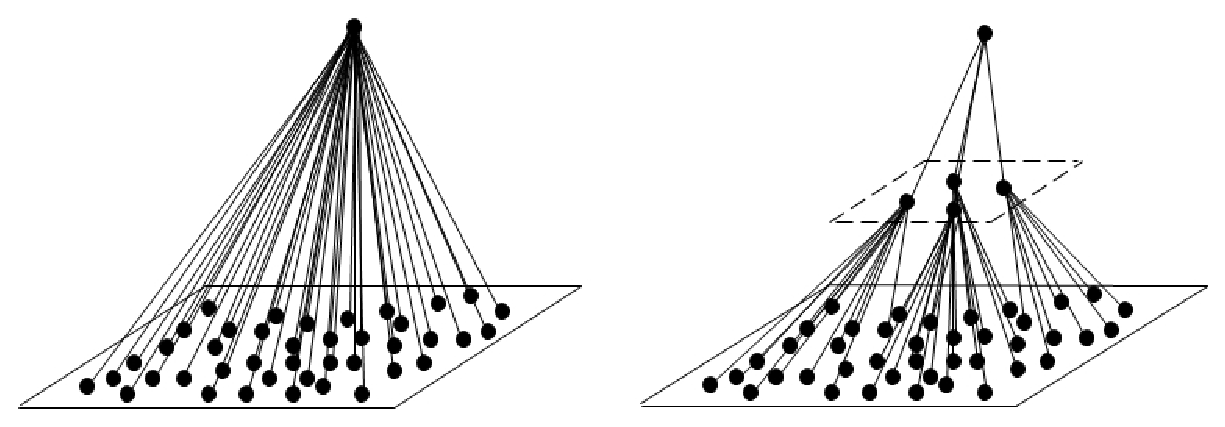
\includegraphics[width=6cm]{compare.eps}
 \caption{Comparatione Times with and without Clustering}
 \label{compare}
\end{figure}

\subsection{Clustering Within the Class with Coupled Similarities}

In this section, a coupled similarities based clustering method will be illustrated. Firstly, by the $Defination$\ref{def:COS}, a coupled similarity between two objects $COS(d_i,d_j)$ can be calculated. After that, for the classification task, we compute the coupled similarities within one class first because we assume there might be more coupled relations within one class than between two classes. In order to enhance the speed of the clustering process, we enumerated all the object within the data set $\mathcal{D}=\{d_{1},d_{2},\ldots,d_{n}\}$ in to a comparison table $Tabel$\ref{tabel} and then calculated the coupled similarities between each of them. Since our definition of similarity is a relative value, it only can be applied when given two objects, which means it cannot create a middle point of two objects. Furthermore, the mean of two categorical attribute cannot be calculated as well, for instance, it is hard to say what gender is between male and female. As a result, the traditional clustering method like K-Means cannot be applied directly, because it couldn't find the mean point within a group of objects. To solve this problem, we used the Spherical K-Means clustering method to instead of K-Means as our clustering method.

\begin{table}
\caption{Coupled Similarity Between Objects}
\centering
\begin{tabular}{|c|c|}
  \hline
  % after \\: \hline or \cline{col1-col2} \cline{col3-col4} ...
  Object Pairs & Similarity\\
  \hline
  $d_{1},d_{2}$ & 0.23 \\
  \hline
  $d_{1},d_{3}$ & 0.31 \\
  \hline
  . & . \\
  . & . \\
  . & . \\
  \hline
  $d_{n},d_{m}$ & $s$ \\
 \hline
\end{tabular}
\label{tabel}
\end{table}

\subsubsection{Spherical K-Means Clustering using Coupled Similarities}
Let $d_{1},d_{2}$ be two categorical object from the data set $\mathcal{D}=\{d_{1},d_{2},\ldots,d_{n}\}$, the similarities among the objects is based on the definition 3.8. The clustering process is to partition the data set $\mathcal{D}$ into $T$ clusters, each of the cluster can be named as $\mathcal{C}=\{c_{1},c_{2},\ldots,c_{t}\}$ respectively. The perfect solution can be formally describe as the following maximization problem:
\begin{equation}
 \{c_{t}\}^{k}_{j=1}=\underset{\{c_{t}\}^{k}_{t=1}}{\operatorname{arg\,max}}\sum^{k}_{t=1}\sum_{d_{i}\in{c_t}}Cos(m_{t},d_{i})
 \end{equation}
 $\{c_{t}\}=\{d_{t1},d_{t2},\ldots,d_{tn}\}$ is a cluster with certain objects, A centroid point $m_{t}$ of cluster ${c_{t}}$ is a object within the $c_{t}$ which has the minimal similarity to all other objects within the cluster, for any object $d'$ in ${c_{t}}$, the centroid point $m_{t}$ that
  \begin{equation}
   \sum_{d_{i}\in{c_{t}}}Cos(m_{t},d_{i})\leq\sum_{d_{i}\in{c_{t}}}Cos(d',d_{i})
 \end{equation}
  The clustering method is straightforward, very similar to K-Means. Firstly, it randomly chooses K object from data set $\mathcal{D}$ as the centroid object ${m_{k}}$, $m$ stands for the temp mode of the cluster and $k$ is the cluster id for each cluster. Secondly, it allocates each object ${d_{n}}$ to theirs nearest centroid object ${m_{k}}$ as a intermediate cluster $c_{k}$, where $c_{k}$ contains a set of objects $\{d_{k1},d_{k2},\ldots,d_{kn}\}$ which are the nearest objects to this centroid object ${m_{k}}$. Thirdly, it searches for a new centroid object within each cluster $c_{k}$, the new centroid object is the object which has minimal similarity to all other object with in the cluster.When the new centroid object has been confirmed, repeat to assign each object to the new centroid object to reform the cluster. Finally, iterate the process until the centroid object is fixed for any cluster $c_{t}$.
     \begin{equation}
   m^{n}_{t}=m^{n+1}_{t}
 \end{equation}
 $n$ stands for the iteration times. Meanwhile, in some extreme case, the centroid object cannot be fixed at all, there is an alternative criterion that
       \begin{equation}
   |(\sum^{k}_{t=1}\sum_{d_{i}\in{c_t}}Cos(m_{t},d_{i}))^{n}- (\sum^{k}_{t=1}\sum_{d_{i}\in{c_t}}Cos(m_{t},d_{i}))^{n+1}|\leq\varepsilon
 \end{equation}
 Same as above $n$ is the iteration times, $\varepsilon$ is the certain threshold, if the "change" of the cluster after iteration is not significant, the searching algorithm will stop.
   The Spherical K-Means clustering method prevents the problems which K-Means leads to, thus it suitable for our coupled similarity based clustering.

\subsubsection{Classification with Coupled Similarities Weighted Cluster Centroid}
For simplify the problem, we take the binary classification task as an example, once the clustering process has been finished, we have several clusters within both positive class $\pi_{A}$ and negative class $\pi_{B}$. Moreover, each centroid of the cluster has its unique value for classification, due to the difference of coupled similarity between them are substantial. The coupled similarity cannot be expressed in the 2D space ,since all the similarities are relative and cannot be drown on one flat picture. However, for simplicity, we use the following figure to illustrated the different similarities between clusters.

\begin{figure}
 \centering
  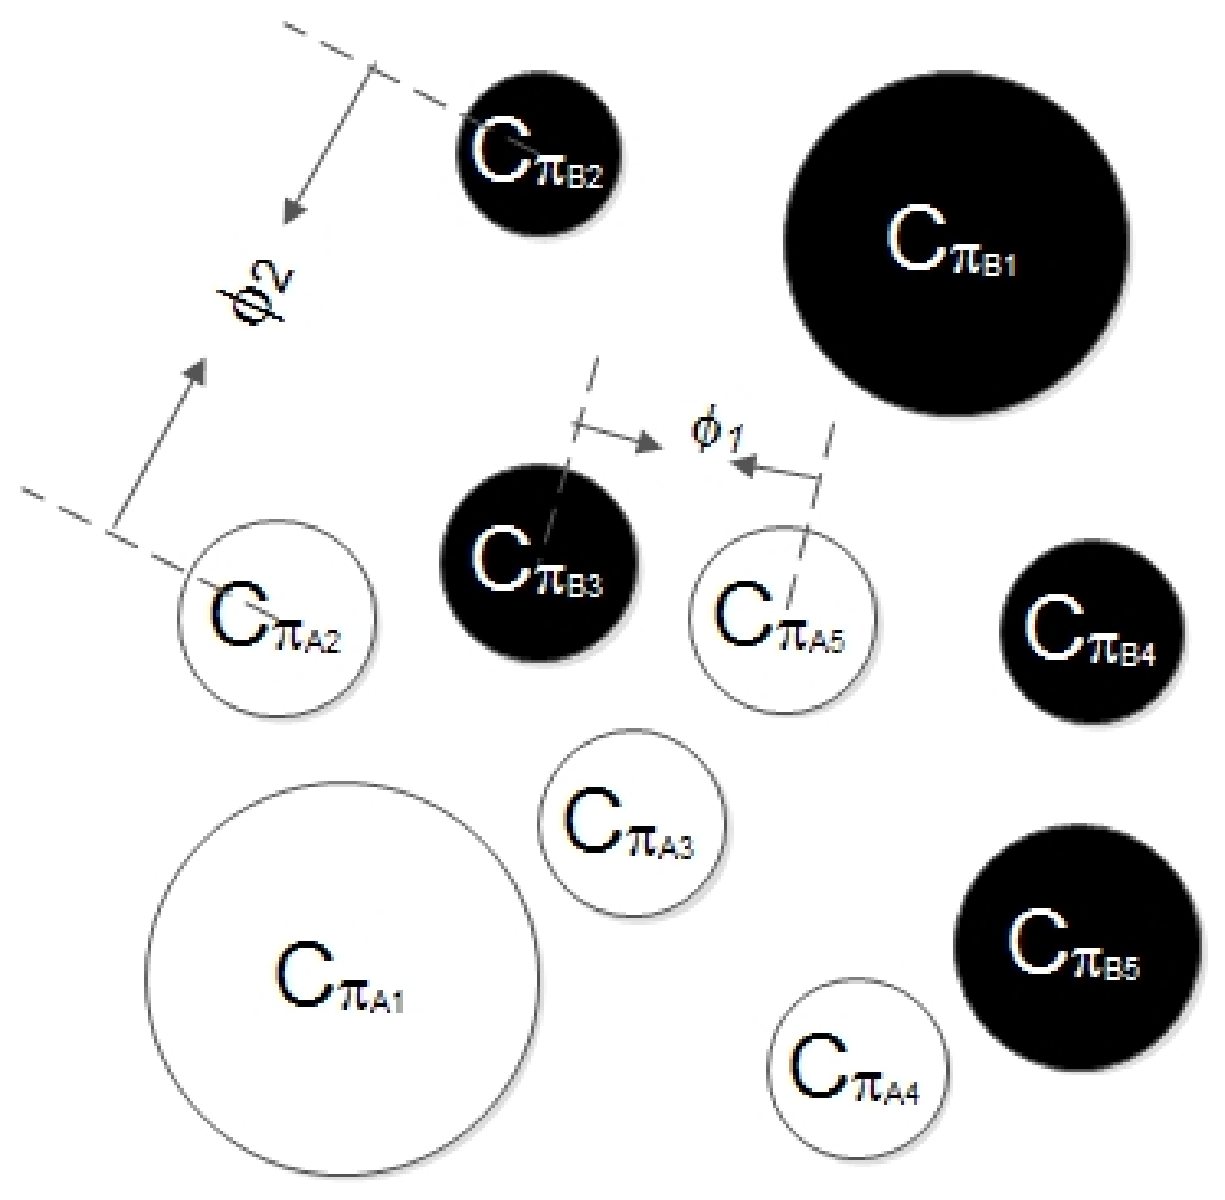
\includegraphics[width=4cm]{cluster.eps}
 \caption{The training data set after clustering}
 \label{cluster}
\end{figure}

As the \ref{cluster} shows, each circular stands for a cluster, and the caption of the circular $C_{\pi_{A}}$ and $C_{\pi_{B}}$ stand for centroid object in both the positive class and negative class respectively, moreover, we also use the different color to present the clusters which belongs to a different class. The $\phi_{1}$ and $\phi_{2}$ is the coupled similarity between two centroid $C_{\pi_{A3}}$ and $C_{\pi_{B5}}$ and $C_{\pi_{A2}}$ and $C_{\pi_{B2}}$. Apparently, the coupled similarity $\phi_{2}$ is significantly larger than $\phi_{1}$. When doing a classification task, the difference of distance will affect the result remarkably. Unfortunately, the classic KNN algorithm neglect this difference and judge every point as equivalent significance. More precisely, when it does a classification job with an incoming object $d_{n}$, and it only counts the amount of the $k$ nearest neighbors $Count(\chi^{k}(d_{n}))$ belong to each class, where the $\chi^{k}(d_{n})$ denote to the set of the nearest neighbors of object $d_{n}$, and if the number of neighbors belong to class A larger than the number of neighbors belong to class B then classified the object to class A, without considering the unique value of each of its neighbors. Let $F$ be the classification function, the classification process of traditional KNN can be describe as:
  \begin{equation}
   F(d_{n})=\left\{
\begin{aligned}
d_{n}\in \pi_{A} &    &   Count(\chi^{k}(d_n)\in\pi_{A})>\\&&Count(\chi^{k}(d_n)\in\pi_{A})\\
d_{n}\in \pi_{B} &    &   Count(\chi^{k}(d_n)\in\pi_{B})>\\&&Count(\chi^{k}(d_n)\in\pi_{A})\\
\end{aligned}
\right.
 \end{equation}
This work proposed a novel classifier with weighted cluster centroid, which comprehensively involved the information of the coupled similarity from every centroid object $C_{\pi_{A}}$ in one class $\pi_{A}$ to all other objects $d_{\pi_{\bar{A}}}^{j}$  belongs to the opposite class $\pi_{\bar{A}}$. The reason is that, by the concept of coupling, every object can be described by others object, which have relation to it. After that this work by utilizing this information to make a certain weight to each centroid object.The computation of coupled similarities weight is quite straightforward:
  \begin{equation}
   W(C_{\pi_{An}})=\sum_{i=1}^{m}\sum_{j=1}^{n}Cos(d_{\pi_{A}}^{i},d_{\pi_{\bar{A}}}^{j})
 \end{equation}
Finally, to classify a incoming object by accumulating the coupled similarities to every centroid object and adding those weights. The classification function is becoming:
  \begin{equation}
   F(d_{n})=\left\{
\begin{aligned}
d_{n}\in \pi_{A} &    &  \sum_{i=1}^{k}W(\chi^{k}(d_n)\in\pi_{A})>  \\
&&\sum_{i=1}^{k}W(\chi^{k}(d_n)\in\pi_{B})\\
d_{n}\in \pi_{B} &    &   \sum_{i=1}^{k}W(\chi^{k}(d_n)\in\pi_{B})>  \\
&&\sum_{i=1}^{k}W(\chi^{k}(d_n)\in\pi_{A})
\end{aligned}
\right.
 \end{equation}

\section{Experiment and Evaluation}
In this section, several experiments are performed on extensive UCI data sets to show the effectiveness and efficiency of our proposed coupled similarities. The experiments are divided into two categories: coupled similarity comparison and \emph{COS} application. For simplicity, we just assign the weight vector $\alpha=(\alpha_k)_{1\times n}$ with values $\alpha(k)=1/n$ in (\ref{eq:IeAVS}).

\subsection{Coupled Similarity Comparison}
 To compare efficiencies, we conduct extensive experiments on the inter-coupled relative similarity metrics: \emph{IRSP}, \emph{IRSU}, \emph{IRSJ}, and \emph{IRSI}. The goal in this set of experiments is to show the obvious superiority of \emph{IRSI}, compared with the most time-consuming measure \emph{IRSP}. As discussed in Section \ref{sec:accuracy}, the computational complexity linearly depends on the time costs of \emph{ICP} with given data. Thus, we consider a comparison of complexities represented by the time costs of \emph{ICP}. Also explained in Section \ref{sec:accuracy}, the complexity for \emph{IRSP} is $O(n^2R^22^R)$, while the other three have equal smaller complexity $O(n^2R^3)$. Here, scalability analysis is explored in terms of these two factors separately: the number of features $|A|$ and the maximal number of attribute values $R$.

\textbf{From the perspective of $|A|$}, Soybean-large data set is considered with $307$ objects and $35$ features. Here, we fix $R$ to be $7$, and focus on $|A|$ ranging from $5$ to $35$ with step $5$. In terms of the total time costs of \emph{ICP}, the computational complexity comparisons among four measures (\emph{IRSP}, \emph{IRSU}, \emph{IRSJ}, and \emph{IRSI}) are depicted in Figure \ref{fig:scalability F}($|A|$). The result indicates that the complexities of all these measures keep increasing when $|A|$ becomes larger. The acceleration of \emph{IRSP} (from $3328$ to $74128$) is the greatest compared with the slightest acceleration of \emph{IRSI} (from $632$ to $15704$). Apart from these two, the scalability curves are almost the same for \emph{IRSU} and \emph{IRSI}, though the complexity of \emph{IRSU} is slightly higher than that of \emph{IRSJ} with varied $|A|$. Therefore, \emph{IRSI} is the most stable and efficient measure to calculate the intra-coupled relative similarity in terms of $|A|$.



\textbf{From the perspective of $R$}, the variation of  $R$ is considered when $|A|$ is confirmed. Here, we take advantage of the Adult data set with $30718$ objects and $13$ features chosen. Specifically, the integer feature ``fnlwgt'' is discretized into different intervals (from 10 to 10000) to form distinct $R$ ranging from 16 to 10000, since one of the existing categorial attributes ``education'' already has 16 values. The outcomes are shown in Figure \ref{fig:scalability F}($R$), in which the horizontal axis refers to $R$, and the vertical axis indicates the relative complexity ratios in terms of $\xi(J/U)$, $\xi(I/J)$, and $\xi(I/U)$. From this figure, we observe all the ratios between $10\%$ and $100\%$, which again verifies the complexity order for these four measures indicated in Section \ref{sec:accuracy}. Another issue is that all three curves decrease as $R$ grows, which means the efficiency advantages of  \emph{IRSJ} upon \emph{IRSU} (from $85.5\%$ to $46.8\%$), \emph{IRSI} upon \emph{IRSJ} (from $78.2\%$ to $40.2\%$), and \emph{IRSI} upon \emph{IRSU} (from $66.9\%$ to $18.8\%$) all become more and more obvious with the increasing of $R$. The general trend of these ratios always falling comes from the fact that there is a higher probability of getting a join set smaller than the whole set, and an intersection set smaller than the join set, with larger $R$. The same conclusion also holds for the ratio $\xi(U/P)$, but this is due to the fact that $q^{-1}(x)=x/2^x$ is a strictly monotonously decreasing function when $x>1$. We omit this ratio in Figure \ref{fig:scalability F}($R$) since the denominator $|ICP^{(P)}|$ becomes exponentially  large when $R$ grows, e.g., it equals to $5.12\times 10^{83}$ when $R=500$. Hence, \emph{IRSI} is the least time-consuming intra-coupled similarity with regard to $R$.

\vspace{0.1cm}
In summary, all the above experiment results clearly show that \emph{IRSI} outperforms \emph{IRSP}, \emph{IRSU}, and \emph{IRSJ} in terms of the computational complexity. In particular, with the increasing numbers of either features or attribute values, \emph{IRSI} demonstrates superior efficiency compared to the others. \emph{IRSJ} and \emph{IRSU} follow, with \emph{IRSP} being the most time-consuming, especially for the large-scale data set.

\subsection{Application}
In this section, we illustrate the performance of this novel method applying on the real world educational data. Educational data mining is a growing hot research topic, many discussion are mentioned about the prediction of the risk that students fail in their subjects. In this work, we used a de-personalized students' demographic data, with 80 demographic features about the student and 400 students in this experimental data. The features include their nationalities, previous education background, previous academic grades, previous scholarship records and much more, not all the features are categorical, if it's numerical we discrete it into 5 equal frequency categorical values. Moreover, the data has been labeled by students previous examination result, if the student is in the top 30 percent of their peers, we labeled it as class A while others we labeled as B. This experiment compared this novel method with some classic classification method by contrasting their the standard classification task metric result, Figure 1 shows that this work has its advantage in most of the metrics. More importantly, the result supported our main concern about the real world data, there are plenty of coupling relation not only between the value of features, but also the among the objects.

\section{Acknowledgment}
This work is sponsored by Australian Research Council Grants (DP1096218, DP0988016, LP100200774, LP0989721), Tianjin Research Project (10JCYBJC07500), and QCIS (Center for Quantum Computation and Intelligent Systems).

\subsection{Citations}

Citations within the text should include the author's last name and
the year of publication, for example~\cite{gottlob:nonmon}.  Append
lowercase letters to the year in cases of ambiguity.  Treat multiple
authors as in the following examples:~\cite{abelson-et-al:scheme}
or~\cite{bgf:Lixto} (for more than two authors) and
\cite{brachman-schmolze:kl-one} (for two authors).  If the author
portion of a citation is obvious, omit it, e.g.,
Nebel~\shortcite{nebel:jair-2000}.  Collapse multiple citations as
follows:~\cite{gls:hypertrees,levesque:functional-foundations}.
\nocite{abelson-et-al:scheme}
\nocite{bgf:Lixto}
\nocite{brachman-schmolze:kl-one}
\nocite{gottlob:nonmon}
\nocite{gls:hypertrees}
\nocite{levesque:functional-foundations}
\nocite{levesque:belief}
\nocite{nebel:jair-2000}

\subsection{Footnotes}

Place footnotes at the bottom of the page in a 9-point font.  Refer to
them with superscript numbers.\footnote{This is how your footnotes
should appear.} Separate them from the text by a short
line.\footnote{Note the line separating these footnotes from the
text.} Avoid footnotes as much as possible; they interrupt the flow of
the text.

\section{Illustrations}

Place all illustrations (figures, drawings, tables, and photographs)
throughout the paper at the places where they are first discussed,
rather than at the end of the paper. If placed at the bottom or top of
a page, illustrations may run across both columns.

Illustrations must be rendered electronically or scanned and placed
directly in your document. All illustrations should be in black and
white, as color illustrations may cause problems. Line weights should
be 1/2-point or thicker. Avoid screens and superimposing type on
patterns as these effects may not reproduce well.

Number illustrations sequentially. Use references of the following
form: Figure 1, Table 2, etc. Place illustration numbers and captions
under illustrations. Leave a margin of 1/4-inch around the area
covered by the illustration and caption.  Use 9-point type for
captions, labels, and other text in illustrations.

\section*{Acknowledgments}

The preparation of these instructions and the \LaTeX{} and Bib\TeX{}
files that implement them was supported by Schlumberger Palo Alto
Research, AT\&T Bell Laboratories, and Morgan Kaufmann Publishers.
Preparation of the Microsoft Word file was supported by IJCAI.  An
early version of this document was created by Shirley Jowell and Peter
F. Patel-Schneider.  It was subsequently modified by Jennifer
Ballentine and Thomas Dean, Bernhard Nebel, and Daniel Pagenstecher.
These instructions are the same as the ones for IJCAI--05, prepared by
Kurt Steinkraus, Massachusetts Institute of Technology, Computer
Science and Artificial Intelligence Lab.

\appendix

\section{\LaTeX{} and Word Style Files}\label{stylefiles}

The \LaTeX{} and Word style files are available on the IJCAI--13
website, {\tt http://www.ijcai-13.org/}.
These style files implement the formatting instructions in this
document.

The \LaTeX{} files are {\tt ijcai13.sty} and {\tt ijcai13.tex}, and
the Bib\TeX{} files are {\tt named.bst} and {\tt ijcai13.bib}. The
\LaTeX{} style file is for version 2e of \LaTeX{}, and the Bib\TeX{}
style file is for version 0.99c of Bib\TeX{} ({\em not} version
0.98i). The {\tt ijcai13.sty} file is the same as the {\tt
ijcai07.sty} file used for IJCAI--07.

The Microsoft Word style file consists of a single file, {\tt
ijcai13.doc}. This template is the same as the one used for
IJCAI--07.

These Microsoft Word and \LaTeX{} files contain the source of the
present document and may serve as a formatting sample.

Further information on using these styles for the preparation of
papers for IJCAI--13 can be obtained by contacting {\tt
pcchair13@ijcai.org}.

%% The file named.bst is a bibliography style file for BibTeX 0.99c
\bibliographystyle{named}
\bibliography{ijcai13}

\end{document}

